\documentclass[tikz, 12pt]{standalone}
\usepackage{tikz}
\usetikzlibrary{calc}
\usetikzlibrary{decorations.pathmorphing}
\tikzset{snake it/.style={decorate, decoration=snake}}
\usepackage{pgfplots} 
\pgfplotsset{compat=1.16}
\usepackage{amsmath}
\usepackage{amssymb}

% Macro for irregular shape
\newcommand\irregularcircle[2]{% radius, irregularity
  \pgfextra {\pgfmathsetmacro\len{(#1)+rand*(#2)}}
  +(0:\len pt)
  \foreach \a in {40,80,...,320}{
    \pgfextra {\pgfmathsetmacro\len{(#1)+rand*(#2)}}
    -- +(\a:\len pt)
  } -- cycle
}

\begin{document}
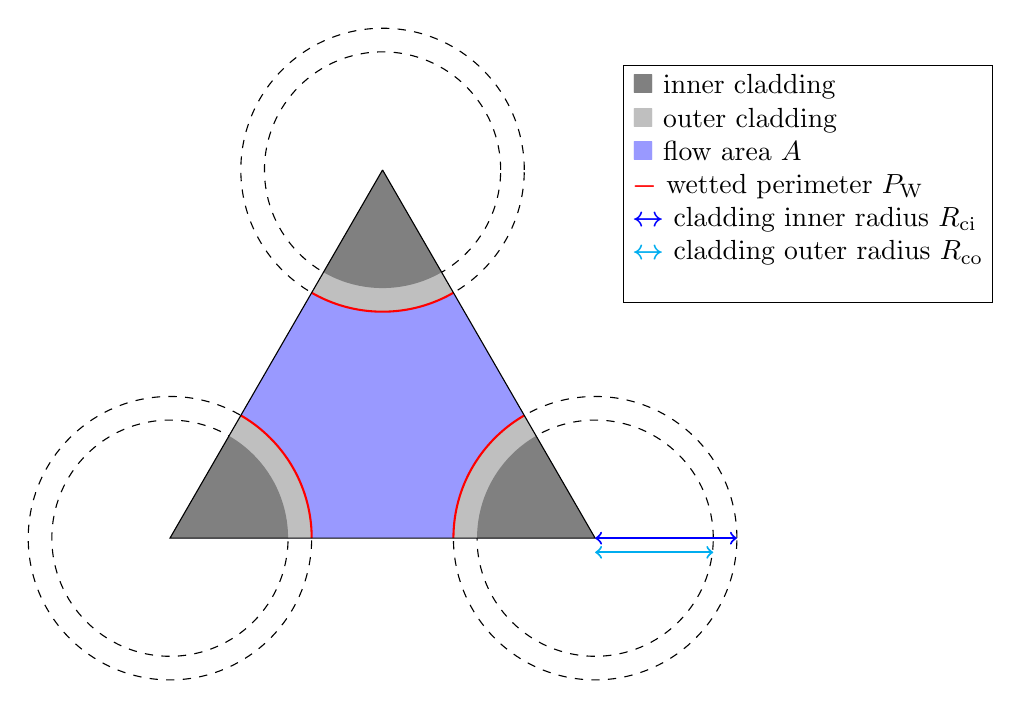
\begin{tikzpicture}[even odd rule]
	\def\r{1.8cm}
	\def\R{1.5cm}
    \coordinate (O1) at (0, 0.866 * 3 * \r) {}; 
    \coordinate (O2) at (-0.5 * 3 * \r, 0 * 3 * \r) {}; 
    \coordinate (O3) at (0.5 * 3 * \r, 0 * 3 * \r) {}; 

    \draw [dashed] (O1) circle (\r);
    \draw [dashed] (O2) circle (\r);
    \draw [dashed] (O3) circle (\r);

    \draw [dashed] (O1) circle (\R);
    \draw [dashed] (O2) circle (\R);
    \draw [dashed] (O3) circle (\R);

	\begin{scope}
    	\clip (O3) -- (O2) -- (O1);
    	\fill [color=blue!40!white] (0, 0) circle (2 * \r);

    	\fill [color=lightgray] (O1) circle (\r);
    	\fill [color=gray] (O1) circle (\R);
    	\draw [color=red, line width=0.75] (O1) circle (\r);
    	\fill [color=lightgray] (O2) circle (\r);
    	\fill [color=gray] (O2) circle (\R);
    	\draw [color=red, line width=0.75](O2) circle (\r);
    	\fill [color=lightgray] (O3) circle (\r);
    	\fill [color=gray] (O3) circle (\R);
    	\draw [color=red, line width=0.75](O3) circle (\r);
	\end{scope}

	\draw (O1) -- (O2) -- (O3) -- (O1);

	\draw[color=blue, <->, line width=0.75] ($(O3) + (0, 0)$) -- ($(O3) + (\r, 0)$);
	\draw[color=cyan, <->, line width=0.75] ($(O3) + (0, -0.1 * \r)$) -- ($(O3) + (\R, -0.1 * \r)$);

	\node[draw,align=left] at (3 * \r, 2.5 * \r) {
		{\color{gray}$\blacksquare$} inner cladding\\
		{\color{lightgray}$\blacksquare$} outer cladding\\
		{\color{blue!40!white}$\blacksquare$} flow area $A$\\
		{\color{red}$\boldsymbol{-}$} wetted perimeter $P_{\textrm{W}}$\\
		{\color{blue}$\boldsymbol{\leftrightarrow}$} cladding inner radius $R_{\textrm{ci}}$\\
		{\color{cyan}$\boldsymbol{\leftrightarrow}$} cladding outer radius $R_{\textrm{co}}$\\
		};



\end{tikzpicture}
\end{document}
